% ============================================================
%  Ballista Investigation — Laboratory Technician Requisition
%  One page A4. Compile: pdflatex lab_tech_ballista.tex
% ============================================================
\documentclass[11pt,a4paper]{article}
\usepackage[T1]{fontenc}
\usepackage[a4paper, top=0.8cm, bottom=0.8cm, left=1.5cm, right=1.5cm]{geometry}
\usepackage{xcolor}
\usepackage{tikz}
\usetikzlibrary{arrows.meta,calc,patterns,decorations.pathreplacing,decorations.markings}
\usepackage{booktabs}
\usepackage{array}
\usepackage{tabularx}
\usepackage{graphicx}
\usepackage{enumitem}
\usepackage[protrusion=true,expansion=false]{microtype}

% ── Colours (muted, print-friendly) ─────────────────────────────────────────
\definecolor{Ink}      {HTML}{1A1A1A}
\definecolor{HeadGrey} {HTML}{333333}
\definecolor{RuleGrey} {HTML}{888888}
\definecolor{BoxGrey}  {HTML}{F0F0F0}
\definecolor{LineGrey} {HTML}{555555}

\setlength{\parindent}{0pt}
\setlength{\parskip}{1pt}
\renewcommand{\arraystretch}{1.12}

% ── Column types ─────────────────────────────────────────────────────────────
\newcolumntype{L}[1]{>{\raggedright\arraybackslash}p{#1}}
\newcolumntype{C}[1]{>{\centering\arraybackslash}p{#1}}

\newcommand{\sechead}[1]{%
  \vspace{0pt}%
  {\bfseries\large\color{HeadGrey} #1}\\[-2pt]
  {\color{RuleGrey}\rule{\linewidth}{0.8pt}}\\[1pt]
}
\newcommand{\cb}{\framebox[1.6ex]{\rule{0pt}{1.4ex}}\hspace{0.4em}}

\begin{document}
\pagestyle{empty}
\small

% ── Title block ──────────────────────────────────────────────────────────────
{\LARGE\bfseries\color{Ink} Laboratory Requisition --- Ballista Investigation}\\[3pt]
{\color{RuleGrey}\rule{\linewidth}{1.2pt}}

\vspace{3pt}
\begin{tabularx}{\linewidth}{@{}X X X@{}}
\textbf{Unit:} Forces \& Motion (Yr 7--8) &
\textbf{Requested by:} \underline{\hspace{3.5cm}} &
\textbf{Date needed:} \underline{\hspace{2.8cm}} \\
\textbf{Lesson:} Projectile investigation &
\textbf{Number of groups:} \underline{\hspace{2cm}} &
\textbf{Period / room:} \underline{\hspace{2.6cm}} \\
\end{tabularx}

% ── Purpose ──────────────────────────────────────────────────────────────────
\sechead{What the students are doing}
Students fire a projectile from a ballista at a \textbf{measured launch angle} from ground level, then film each shot in slow motion. From the video they measure the total time of flight and the maximum height reached, and from the floor they measure the horizontal range ($R$). They use this to calculate gravity ($g$). Each group runs \textbf{10 shots}, so allow 50--60 minutes. \emph{Note: unlike the trebuchet (high arc, horizontal launch), the ballista is fired at an adjustable angle from the ground.}

% ── Equipment table ──────────────────────────────────────────────────────────
\sechead{Equipment required}
\begin{tabularx}{\linewidth}{@{}c L{6.3cm} c c X@{}}
\toprule
\textbf{\cb} & \textbf{Item} & \textbf{Per group} & \textbf{Total needed} & \textbf{Notes} \\
\midrule
\cb & Ballista (torsion or elastic) & 1 & \rule{1.5cm}{0.4pt} & Class set, or shared between groups \\
\cb & Projectile & 1 & \rule{1.5cm}{0.4pt} & 40\,g foam dart or soft ball; \textbf{identical} for all groups \\
\cb & Spare projectiles & 2 & \rule{1.5cm}{0.4pt} & Same mass --- in case of loss \\
\cb & Protractor (large) or angle gauge & 1 & \rule{1.5cm}{0.4pt} & To set \& read the launch angle \\
\cb & Measuring tape (5\,m+) & 1 & \rule{1.5cm}{0.4pt} & For measuring range $R$ \\
\cb & Metre ruler & 1 & \rule{1.5cm}{0.4pt} & For scale reference in video \\
\cb & Spirit level & 1 & \rule{1.5cm}{0.4pt} & To check the ballista base is level \\
\cb & Masking tape & 1 roll & \rule{1.5cm}{0.4pt} & Mark launch line + exclusion zone \\
\cb & Smartphone or tablet + tripod & 1 & \rule{1.5cm}{0.4pt} & Must shoot slow motion ($\geq$120\,fps) \\
\cb & Safety glasses & 4 & \rule{1.5cm}{0.4pt} & One per student --- \textbf{mandatory} \\
\bottomrule
\end{tabularx}

% ── Setup + Safety side by side ───────────────────────────────────────────────
\begin{minipage}[t]{0.50\linewidth}
\sechead{Setup before lesson}
\begin{enumerate}[itemsep=0pt, leftmargin=1.4em, topsep=0pt]
  \item Place each ballista on a level surface at one end of a clear run; check the base with a spirit level.
  \item Mark the \textbf{launch line} on the floor with tape, directly below the projectile's starting position. Label it \textbf{``0\,m''}.
  \item Lay the measuring tape along the floor from the ``0\,m'' line toward the landing zone.
  \item Attach or stand a protractor at the pivot so students can set and read the launch angle.
  \item Place a metre ruler upright near the flight path (visible in video) as a scale reference.
  \item Mark a \textbf{2\,m exclusion zone} in front of each ballista with tape.
  \item Confirm each camera is charged and slow-motion mode is on.
\end{enumerate}
\end{minipage}
\hfill
\begin{minipage}[t]{0.46\linewidth}
\sechead{Safety}
\begin{itemize}[itemsep=0pt, leftmargin=1.4em, topsep=0pt, label=\textbullet]
  \item \textbf{Risk level: Medium.} Teacher supervises all shots.
  \item Use only \textbf{soft / foam projectiles} --- never hard or pointed objects.
  \item Safety glasses worn by all students during firing.
  \item Only one person fires each ballista; others stand \textbf{behind} it.
  \item Nobody in front of or beside the firing line.
  \item Never aim toward people --- aim down the marked range only.
  \item Projectiles retrieved only on teacher's ``all clear''.
  \item Firing mechanism reset and locked before reloading.
\end{itemize}
\end{minipage}


% ── Footer on page 1 ─────────────────────────────────────────────────────────
\vspace{4pt}
{\color{RuleGrey}\rule{\linewidth}{0.8pt}}
{\footnotesize
\textbf{Notes / queries for teacher:} \underline{\hspace{7.5cm}}
\hfill \textbf{Prepared by (tech):} \underline{\hspace{3.5cm}}}

\vfill
\begin{center}
{\footnotesize\itshape\color{RuleGrey} Setup diagram overleaf $\rightarrow$}
\end{center}

% ============================================================================
%  PAGE 2 — FULL-SIZE SETUP DIAGRAM
% ============================================================================
\clearpage

{\LARGE\bfseries\color{Ink} Ballista --- Station Setup Diagram}\\[3pt]
{\color{RuleGrey}\rule{\linewidth}{1.2pt}}

\vspace{4pt}
{\color{LineGrey} Plan view of one ballista station. Set up each station as shown below. All distances are
examples --- actual values depend on the ballista and launch angle used.}

\vspace{12pt}

\begin{center}
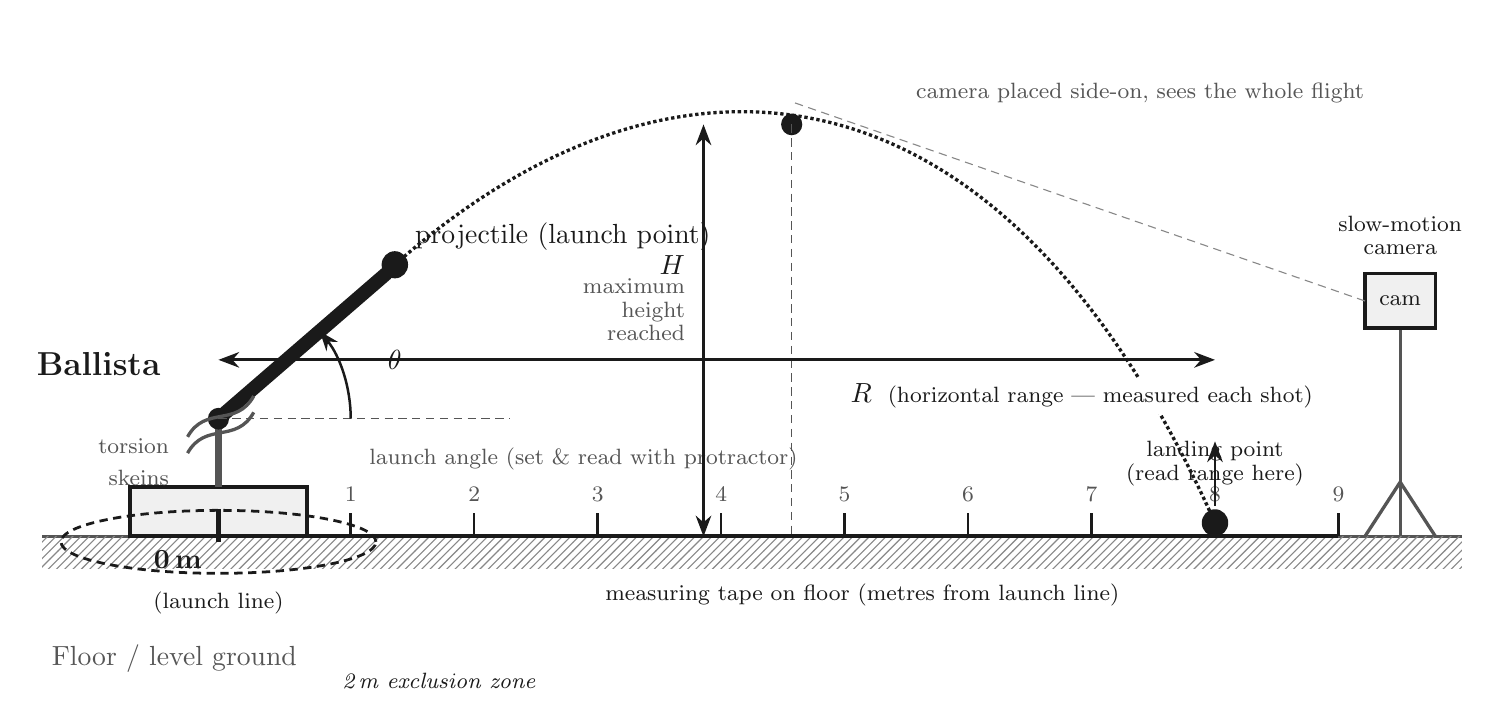
\begin{tikzpicture}[font=\normalsize, x=1.12cm, y=1.15cm]

  % ===== FLOOR =====
  \draw[line width=1.2pt, LineGrey] (-0.5,0) -- (15.6,0);
  \fill[pattern=north east lines, pattern color=RuleGrey]
        (-0.5,-0.35) rectangle (15.6,0);
  \node[anchor=west, text=LineGrey] at (-0.5,-1.35) {Floor / level ground};

  % ===== BALLISTA (left, firing at an angle) =====
  % base
  \draw[line width=1.4pt, Ink, fill=BoxGrey] (0.5,0) rectangle (2.5,0.55);
  % stand / pivot post
  \draw[line width=2.4pt, LineGrey] (1.5,0.55) -- (1.5,1.3);
  \fill[Ink] (1.5,1.3) circle (0.12);
  % launch arm/rail at ~40 degrees
  \draw[line width=5pt, Ink, line cap=round] (1.5,1.3) -- (3.4,2.9);
  % torsion skeins (twisted bundles) at base of arm
  \draw[line width=1.2pt, LineGrey] (1.15,1.1) .. controls (1.35,1.45) and (1.7,1.2) .. (1.9,1.55);
  \draw[line width=1.2pt, LineGrey] (1.15,0.92) .. controls (1.35,1.27) and (1.7,1.02) .. (1.9,1.37);
  \node[anchor=east, text=LineGrey, font=\footnotesize] at (1.05,1.0) {torsion};
  \node[anchor=east, text=LineGrey, font=\footnotesize] at (1.05,0.65) {skeins};
  % projectile at end of rail (launch point)
  \fill[Ink] (3.5,3.0) circle (0.15);
  \node[anchor=south west, text=Ink] at (3.62,3.05) {projectile (launch point)};
  \node[anchor=east, text=Ink, font=\bfseries\large] at (0.95,1.9) {Ballista};

  % ===== LAUNCH ANGLE =====
  \draw[densely dashed, LineGrey] (1.5,1.3) -- (4.8,1.3);
  \draw[-{Stealth}, line width=0.9pt, Ink] (3.0,1.3) arc (0:40:1.5);
  \node[text=Ink, font=\bfseries] at (3.5,1.95) {$\theta$};
  \node[anchor=west, text=LineGrey, font=\footnotesize] at (3.1,0.85)
        {launch angle (set \& read with protractor)};

  % ===== TRAJECTORY (full parabola) =====
  \draw[line width=1.2pt, Ink, densely dotted]
        (3.5,3.0) .. controls (6.5,5.6) and (10.3,5.6) .. (12.8,0.15);

  % ===== MAX HEIGHT H =====
  \coordinate (apex) at (8.0,4.55);
  \fill[Ink] (apex) circle (0.12);
  \draw[densely dashed, LineGrey] (apex) -- (8.0,0);
  \draw[{Stealth}-{Stealth}, line width=1pt, Ink] (7.0,0) -- (7.0,4.55);
  \node[anchor=east, text=Ink, font=\bfseries] at (6.9,3.0) {$H$};
  \node[anchor=east, text=LineGrey, font=\footnotesize, align=right] at (6.9,2.5)
        {maximum\\[-1pt]height\\[-1pt]reached};

  % ===== MEASURING TAPE =====
  \draw[line width=1.4pt, Ink] (1.5,0) -- (14.2,0);
  \draw[line width=1.6pt, Ink] (1.5,-0.06) -- (1.5,0.3);
  \node[anchor=north east, text=Ink, font=\bfseries] at (1.42,-0.05) {0\,m};
  \node[anchor=north, text=Ink, font=\footnotesize] at (1.5,-0.5) {(launch line)};
  \foreach \x/\lab in {3.0/1,4.4/2,5.8/3,7.2/4,8.6/5,10.0/6,11.4/7,12.8/8,14.2/9}{
    \draw[line width=0.9pt, Ink] (\x,0) -- (\x,0.26);
    \node[anchor=south, text=LineGrey, font=\footnotesize] at (\x,0.28) {\lab};
  }
  \node[anchor=north, text=Ink, font=\footnotesize] at (8.8,-0.42)
        {measuring tape on floor (metres from launch line)};

  % ===== LANDING POINT =====
  \fill[Ink] (12.8,0.15) circle (0.15);
  \draw[{Stealth}-, line width=1pt, Ink] (12.8,1.05) -- (12.8,0.34);
  \node[anchor=south, text=Ink, align=center, font=\footnotesize] at (12.8,0.45)
        {landing point\\[-1pt](read range here)};

  % ===== RANGE R =====
  \draw[{Stealth}-{Stealth}, line width=1pt, Ink] (1.5,1.95) -- (12.8,1.95);
  \node[anchor=west, text=Ink, fill=white, inner sep=2pt, font=\bfseries] at (8.6,1.55)
        {$R$ \,\normalfont\footnotesize(horizontal range --- measured each shot)};

  % ===== CAMERA =====
  \draw[line width=1.2pt, LineGrey] (14.9,0) -- (14.9,2.3);
  \draw[line width=1.2pt, LineGrey] (14.5,0) -- (14.9,0.6) -- (15.3,0);
  \draw[line width=1.2pt, Ink, fill=BoxGrey] (14.5,2.3) rectangle (15.3,2.9);
  \node[text=Ink, font=\footnotesize] at (14.9,2.6) {cam};
  \node[anchor=south, text=Ink, align=center, font=\footnotesize] at (14.9,3.0)
        {slow-motion\\[-1pt]camera};
  \draw[densely dashed, RuleGrey] (14.5,2.6) -- (8.0,4.8);
  \node[text=LineGrey, font=\footnotesize, anchor=west] at (9.3,4.9)
        {camera placed side-on, sees the whole flight};

  % ===== EXCLUSION ZONE =====
  \draw[densely dashed, line width=1pt, Ink]
        (1.5,-0.06) ellipse (2.0cm and 0.4cm);
  \node[text=Ink, font=\footnotesize, anchor=north] at (4.0,-1.4)
        {\itshape 2\,m exclusion zone};

\end{tikzpicture}
\end{center}

\vspace{18pt}

% ── Key / legend as a clean table ────────────────────────────────────────────
\sechead{Key to the diagram}
\begin{tabularx}{\linewidth}{@{}p{1.4cm} X@{}}
\textbf{$\theta$} & Launch angle --- set and read with a protractor mounted at the pivot. This is the variable students change between sets of shots. \\
\textbf{$H$} & Maximum height the projectile reaches --- read from the slow-motion video against the upright metre ruler used as a scale reference. \\
\textbf{$R$} & Horizontal range --- distance from the ``0\,m'' launch line to where the projectile lands, read off the measuring tape after each shot. \\
\textbf{Camera} & Positioned side-on at a fixed distance so the whole flight path is in frame. Students count video frames to find the time of flight and the time to reach peak height. \\
\textbf{Skeins} & The twisted rope bundles (or elastic) that store the launching energy. Keep tension/twist identical between shots within a group. \\
\end{tabularx}

\vspace{10pt}
{\color{RuleGrey}\rule{\linewidth}{0.8pt}}
{\footnotesize\itshape\color{LineGrey} One station shown. Replicate this layout for each group, leaving clear space between stations and down each firing lane.}

\end{document}
